%oneside para una impresi\'on simple.
%titlepage define que vamos a tener una portada.
%openany para que los cap\'{\i}tulos empiecen en cualquier p\'agina y no s\'olo las impares.
%final es para compilar a modo normal. Cambiar a draft para que se compile en modo borrador. No se pone final dado que viene por defecto.
\documentclass[a4paper, 12pt, oneside, titlepage, openany]{book}

% Para el seccionado, debe colocarse al principio este package.
\usepackage{titlesec}

% Encoding + cmap (para obtener un mapeo UTF8 adecuado)
\usepackage{cmap}
\usepackage[utf8]{inputenc}
\usepackage[T1]{fontenc} % Para poder copiar y pegar el texto desde un pdf
\usepackage{lmodern}

\usepackage[backend=biber, style=iso-authoryear, language=spanish]{biblatex}
\DeclareUnicodeCharacter{202F}{~} % Para reemplazar el caracter 202F por un espacio
\bibliography{biblio.bib}
\setcounter{tocdepth}{3}
\setcounter{secnumdepth}{3}
% Esto último es para la cantidad de niveles en el índice

\DeclareFieldFormat{urldate}{\mkbibbrackets{consultado\space#1}}

% Para colores
\usepackage[usenames,dvipsnames]{xcolor}

% Para flotar figuras y tablas
\usepackage{framed}

% Para asegurar que las figuras y tablas queden en la secci\'on correspondiente
\usepackage[section,above,below]{placeins}

% Para microtipograf\'{\i}a
\usepackage{microtype}

% Permite tama\~no de fuentes arbitrarios
\usepackage{anyfontsize}

% Itemize
\usepackage{enumitem}
\newlist{Properties}{enumerate}{2}
\setlist[Properties]{label=Propiedad \arabic*.,itemindent=*}
\renewcommand{\labelitemii}{\textasteriskcentered}
\renewcommand{\labelitemiii}{-}

\usepackage{lastpage} % Para poder contar las p\'aginas, habilita el \pageref command.
\usepackage{titleps} % Para la tabla de contenidos
\usepackage{textcase}
\usepackage{pdfpages}
\usepackage{float}
\usepackage{caption}
\usepackage{booktabs}

% \parbox[b] es para poner texto sobre el bottom
\newpagestyle{ruled}{
	\sethead{
\includegraphics[width=3.7cm]{./images/UADE_LARGE}}
			{\parbox[b]{0.43\textwidth}{\raggedright\MakeUppercase{Título de la PFI}}}
			{
				\raisebox{1.5ex}{%
					\parbox[b]{0.26\textwidth}{\raggedleft
					\begin{tabular}{r}
						Navarrete, Ezequiel \\
					\end{tabular}
					}
				}
			}\headrule{}
	\setfoot[][][P\'agina \thepage\ de~\pageref*{LastPage}]{}{}{P\'agina \thepage\ de~\pageref*{LastPage}}\footrule{}
}
\pagestyle{ruled}

% Para que la primera página de cada capítulo no sea tratada como especial
\makeatletter
\let\ps@plain\ps@ruled
\makeatother

% M\'argenes
\usepackage{vmargin}
\setmarginsrb{2.7cm}{2cm}{2.3cm}{1.5cm}{0cm}{2cm}{0cm}{1cm}

% Se pide numeraci\'on de tablas en n\'umeros romanos
\renewcommand{\thetable}{\thechapter.\Roman{table}}

% Espaciado antes y despu\'es de una figura respecto del texto
\setlength{\textfloatsep}{5pt}

% Para notas
\usepackage{todonotes}
\setlength{\marginparwidth}{2cm}
\newcommand{\Nico}[1]{\todo[color=green!30,inline]{\textbf{Nico:} #1}}
\newcommand{\Fermat}[1]{\todo[color=green!30]{\textbf{Fermat:} #1}}

% Espaciado entre referencias en la bibliograf\'{\i}a
\usepackage{etoolbox}
\patchcmd{\thebibliography}
  {\settowidth}
  {\setlength{\itemsep}{6pt}\settowidth}
  {}{}
\apptocmd{\thebibliography}
  {\small}
  {}{}

\usepackage[spanish,es-nodecimaldot]{babel}
\usepackage{csquotes}
\addto\captionsspanish{
	\renewcommand{\contentsname}{\'Indice}
	\renewcommand{\listfigurename}{Lista de Figuras}
	\renewcommand{\listtablename}{Lista de Tablas}
	\renewcommand{\tablename}{TABLA}
}

% Para que el primer parrafo de un cap\'{\i}tulo tenga identado.
\usepackage{indentfirst}
\setlength{\parindent}{36pt}

% Para tablas complejas
\usepackage{multicol,multirow}
\usepackage{array,longtable}

% Times New Roman para texto y matemáticas. Debe ir antes de los paquetes AMS.
\usepackage{mathptmx}

\usepackage{amsmath,amsfonts,amssymb,amsthm}

\allowdisplaybreaks{}

\usepackage{cancel}

\newenvironment{example}[1][Ejemplo]{\begin{trivlist}
	\item[\hspace{\labelsep} {\itshape{} #1}]}{\end{trivlist}}

\newenvironment{examples}[1][Ejemplos]{\begin{trivlist}
	\item[\hspace{\labelsep} {\itshape{} #1}]}{\end{trivlist}}

\newenvironment{EstadoDelArte}
    {\small\begin{center}
    \bfseries{EstadoDelArte} \end{center}}

\newenvironment{Enfoque metodologico}
    {\small\begin{center}
    \bfseries{Enfoque metodologico} \end{center}}

\newenvironment{Cronograma}
    {\small\begin{center}
    \bfseries{Cronograma} \end{center}}

\input{config/symbols}

\usepackage[normalem]{ulem}

\usepackage{setspace}
\onehalfspacing

% En UADE no existe la noción de capítulo en la tesis, por más que en LaTeX sí lo tratemos como tal.
% Además nos piden que el tamaño de letra de lo que para nosotros es una sección, subsección y demás, sean del mismo tamaño.
\titleformat{\chapter}
  {\bfseries\fontsize{14pt}{14pt}\selectfont}
  {\thechapter}{1em}{}
\titlespacing*{\chapter}{0pt}{12pt}{6pt}

\titleformat{\section}
  {\bfseries\fontsize{14pt}{14pt}\selectfont}
  {\thesection}{1em}{}
\titlespacing*{\section}{0pt}{12pt}{6pt}

\titleformat{\subsection}
  {\bfseries\fontsize{14pt}{14pt}\selectfont}
  {\thesubsection}{1em}{}
\titlespacing*{\subsection}{0pt}{12pt}{6pt}

\titleformat{\subsubsection}
  {\bfseries\fontsize{14pt}{14pt}\selectfont}
  {\thesubsubsection}{1em}{}
\titlespacing*{\subsubsection}{0pt}{12pt}{6pt}

% -> Acá se empieza a modificar el tamaño de los títulos autogenerados, como los de las listas de figuras y tablas
\usepackage{tocloft}
\cftsetindents{table}{0em}{4em}

\renewcommand{\cfttoctitlefont}{\bfseries\fontsize{14pt}{16pt}\selectfont}
\setlength{\cftbeforetoctitleskip}{12pt}
\setlength{\cftaftertoctitleskip}{6pt}

% Fuente del título (14pt, negrita)
\renewcommand{\cftloftitlefont}{\bfseries\fontsize{14pt}{16pt}\selectfont}
\renewcommand{\cftlottitlefont}{\bfseries\fontsize{14pt}{16pt}\selectfont}

% Espaciado antes y después del título
\setlength{\cftbeforeloftitleskip}{12pt}
\setlength{\cftafterloftitleskip}{6pt}
\setlength{\cftbeforelottitleskip}{12pt}
\setlength{\cftafterlottitleskip}{6pt}

% IMPORTANTE: En la entrega final de UADE se debe dejar sin color.
% Para trabajar:
\usepackage[
	colorlinks=true,
	citecolor=red,
	linkcolor=red,
	urlcolor=blue
]{hyperref}

% pdfcomment debe ir después de hyperref para evitar problemas con enlaces internos.
\usepackage{pdfcomment}

% Para la entrega final:
%\usepackage[hidelinks]{hyperref}
%\hypersetup{
%    colorlinks=false,
%    pdfborder={0 0 0},
%    linktoc=none
%}

\DefineBibliographyStrings{spanish}{
  online   = {En línea},
  urlfrom  = {Disponible en:},
  andothers = {\mkbibemph{et\addabbrvspace al\adddot}}
}

\begin{document}

% Se desactivan los anchors solo para la portada PDF externa.
% Esto evita que los enlaces internos apunten por error a la portada.
\hypersetup{pageanchor=false}

\clearpage
\thispagestyle{empty}

\includepdf[
  pages=1,
  scale=1.01,
  offset=25mm -25mm,
  pagecommand={\thispagestyle{empty}},
  noautoscale,
  trim=0 0 0 0,
  clip
]{cover/portadaPFI.pdf}

\clearpage

\begin{titlepage}
    \centering

    {\textbf{\fontsize{18}{20}\selectfont PROYECTO FINAL DE INGENIERÍA} \par}
    \vspace{1.5cm}

    {\textbf{\fontsize{16}{18}\selectfont Sistema de análisis del movimiento del tren inferior basado en inteligencia artificial para la detección de patrones de riesgo de lesiones en fútbol} \par}
    \vspace{0.5cm}

    {\textbf{\fontsize{14}{16}\selectfont Navarrete, Ezequiel -- LU 1109716} \par}
    {\fontsize{14}{16}\selectfont Ingeniería Informática \par}
    \vspace{1.5cm}

    {\fontsize{14}{16}\selectfont Tutor: \par}
    {\textbf{\fontsize{14}{16}\selectfont Sacco, Andrés Damian,
		\\ (UADE) Universidad Argentina de la Empresa Lima 757, Cdad. Autónoma de Buenos Aires, Argetina.
			} \par}
    \vspace{3cm}

	{\textbf{\fontsize{14}{16}\selectfont \the\year} \par}
    % {\textbf{\fontsize{14}{16}\selectfont 13 de Junio de 2026} \par} % se puede hardcodear
	% {\textbf{\fontsize{14}{16}\selectfont \today} \par} % fecha completa si es la entrega final
    \vspace{2cm}

    
\includegraphics[width=0.30\textwidth]{./images/UADE}\par \vspace{1cm}
    {\textbf{\fontsize{14}{16}\selectfont UNIVERSIDAD ARGENTINA DE LA EMPRESA} \par}
    {\fontsize{14}{16}\selectfont FACULTAD DE INGENIERÍA Y CIENCIAS EXACTAS \par}
\end{titlepage}
%\input{chapters/acknowledgments}

\newpage
\input{chapters/summary}

\newpage
\input{chapters/abstract}

\newpage
\tableofcontents

\clearpage

% A partir de acá se activan los enlaces internos del documento.
\hypersetup{pageanchor=true}

\pagenumbering{arabic}
\setcounter{page}{1}

\chapter{Introducción}

\section{Objetivo}

Completar.

\section{Alcance}

Completar.

\section{Descripción}

Completar.

\chapter{Antecedentes}\label{antecedentes}

\section{Marco teórico}

En esta sección se presenta la base teórica necesaria para entender el problema que se plantea. 
Para ello, se introducen los conceptos principales para comprender las lesiones deportivas, 
sus características generales y cómo impactan particularmente en el fútbol argentino. 
Luego, se profundiza en las lesiones deportivas en el tren inferior, con especial atención en la rodilla y 
el tobillo, para luego avanzar con conceptos de prevención de lesiones, con el objetivo de comprender qué 
aspectos pueden ser considerados para el análisis del movimiento. Por último, se presentan los conceptos 
tecnológicos que sustentan este proyecto, incluyendo inteligencia artificial aplicada al deporte, 
visión por computadora, estimación de postura humana y aprendizaje automático aplicado al análisis de movimiento.

\subsection{Lesiones deportivas en fútbol}

El fútbol, también conocido como soccer, es una disciplina que se caracteriza por una alta demanda física y de coordinación.
Durante su práctica, los jugadores realizan acciones como carreras, saltos, aceleraciones, desaceleraciones, cambios bruscos de dirección y contacto físico. 
Esta combinación de esfuerzos convierte al fútbol en un deporte con exposición frecuente a lesiones musculoesqueléticas\footnote{Lesiones musculoesqueléticas: lesiones que afectan músculos, huesos, articulaciones, ligamentos o tendones.}, 
tanto en contextos competitivos como durante los entrenamientos.

Las lesiones deportivas en fútbol pueden afectar la continuidad de la práctica, el rendimiento del jugador y su bienestar físico.
Al tratarse de un deporte dinámico, con acciones de alta intensidad y situaciones de oposición constante, los futbolistas están 
expuestos a distintos tipos de lesiones que pueden producirse tanto durante los partidos como en las sesiones de entrenamiento. 
Según \textcite{PfirrmannEtAl2016}, en futbolistas masculinos profesionales adultos se identificó que las tasas de lesión 
son mayores durante los partidos que durante los entrenamientos, aunque ambos contextos representan situaciones relevantes 
de exposición al riesgo. Además, el mismo trabajo indica que las lesiones en el fútbol se concentran principalmente en los miembros inferiores.

Este predominio puede explicarse por la propia dinámica del deporte, donde gran parte de las acciones dependen del desplazamiento, los apoyos, 
la carrera, los cambios de dirección y el golpeo de la pelota. Por este motivo, el análisis de las lesiones en fútbol suele prestar especial 
atención a las piernas, rodillas, tobillos y pies.

Además del impacto físico y deportivo, algunas lesiones pueden implicar períodos prolongados de recuperación, interrupción de la actividad 
y costos asociados al tratamiento y la rehabilitación. En este sentido, estos tratamientos pueden generar una carga económica relevante,
debido a los costos médicos, la rehabilitación y el tiempo de inactividad deportiva \parencite{RossEtAl2023}.

\subsection{Lesiones en el fútbol profesional argentino}

En Argentina, el fútbol ocupa un lugar destacado dentro de las prácticas deportivas y recreativas.
Según la Encuesta Nacional sobre Actividad Física y Deporte 2023, el fútbol fue el deporte más
practicado entre las personas encuestadas que realizaban actividad física o deportiva de manera
habitual, con un 41,3\%. Este dato permite dimensionar la relevancia social y deportiva de la
disciplina en el país, no solo en el ámbito profesional, sino también en espacios recreativos
\parencite{ObservatorioSocialDeporte2023}. Estos datos se presentan en la Tabla~\ref{tab:deportes-practicados}.

A partir de esta relevancia, el análisis de las lesiones asociadas al fútbol argentino resulta
especialmente pertinente. Si bien gran parte de la literatura epidemiológica\footnotemark sobre lesiones en
fútbol proviene de contextos europeos o de ligas de alto rendimiento internacional, también existen
estudios locales que permiten aproximarse a la realidad argentina. En un estudio realizado sobre
un equipo profesional del fútbol argentino durante dos temporadas, se observó una elevada
prevalencia de lesiones y una mayor incidencia durante los partidos en comparación con los
entrenamientos \parencite{BaldjianEtAl2022}.

El mismo trabajo identificó que las lesiones más frecuentes fueron la lesión muscular estructural
del bíceps femoral y el esguince lateral de tobillo. Sin embargo, las lesiones del ligamento
cruzado anterior se destacaron por su mayor impacto, debido al tiempo de ausencia que generan
\parencite{BaldjianEtAl2022}. En línea con esta problemática, un análisis reciente sobre jugadores
profesionales argentinos durante la temporada 2023-2024 también señala a las roturas de ligamentos
cruzados como un fenómeno relevante dentro del fútbol local, con tiempos de recuperación
prolongados \parencite{BaezBanegasEtAl2024}.

\footnotetext{Epidemiología: rama de la medicina que estudia la distribución, frecuencia y factores determinantes de enfermedades o lesiones en poblaciones humanas.}

\begin{table}[H]
\centering
\caption{Deportes practicados en Argentina según ENAFYD 2023}
\label{tab:deportes-practicados}
\begin{tabular}{lc}
\toprule
\textbf{Deporte} & \textbf{\%} \\
\midrule
Fútbol & 41,3 \\
Natación & 15,8 \\
Vóley & 13,9 \\
Básquet & 9,3 \\
Boxeo & 8,1 \\
Pádel & 6,9 \\
Tenis & 5,5 \\
Patín / roller & 5,4 \\
Rugby & 5,2 \\
\bottomrule
\end{tabular}
\caption*{Fuente: elaboración propia a partir de la Encuesta Nacional sobre Actividad Física y Deporte 2023.}
\end{table}

\subsection{Lesiones por torsión en el tren inferior}

Las lesiones por torsión en el tren inferior se producen cuando una o varias articulaciones son
sometidas a fuerzas rotacionales o a una combinación de cargas que superan su capacidad de
estabilización, como mencionan \textcite{ShimokochiShultz2008}. Este tipo de mecanismo puede
aparecer durante acciones en las que el pie permanece apoyado sobre el suelo mientras el resto
del cuerpo continúa desplazándose o cambia de dirección. En estas situaciones, la carga no
actúa únicamente en una dirección, sino que puede combinar flexión, extensión, rotación,
desplazamientos laterales y fuerzas de compresión.

Durante la práctica deportiva, el pie y el tobillo cumplen un papel relevante en la relación
entre el cuerpo y el suelo. El tobillo actúa como un puente de contacto entre el cuerpo y el
pie, mientras que el pie permite un vínculo dinámico con la superficie de apoyo. Por este
motivo, las cargas que se generan durante gestos como la carrera, el salto, el apoyo o el cambio
de dirección pueden afectar la forma en que se distribuyen las fuerzas en el miembro inferior
\parencite{SanchezHernandezEtAl2016}.

En el caso del pie y el tobillo, la literatura describe una relación entre los movimientos del
pie, la movilidad de la articulación subastragalina\footnote{La articulación subastragalina,
también denominada subtalar, se encuentra entre el astrágalo y el calcáneo. Participa en
movimientos del pie como la inversión y la eversión, y contribuye a la adaptación del pie al
terreno.} y los movimientos rotacionales de la tibia y el astrágalo\footnote{El astrágalo es un
hueso del tobillo ubicado entre la tibia, el peroné y el calcáneo. Transmite cargas entre la
pierna y el pie, y participa en los movimientos del tobillo.}. La pronación del pie se acompaña
de rotación interna de la tibia, mientras que la supinación se asocia con rotación externa como
se observa en la Figura~\ref{fig:movimiento-tibia-antepie}, esta relación permite visualizar
cómo los movimientos del pie pueden acompañarse de movimientos rotacionales de la tibia. Esta
relación muestra que los movimientos del pie no deben analizarse de forma aislada, ya que pueden
influir en la alineación del resto del miembro inferior durante gestos de apoyo, carrera, salto
o cambio de dirección \parencite{SanchezHernandezEtAl2016}.

\begin{figure}[H]
    \centering
    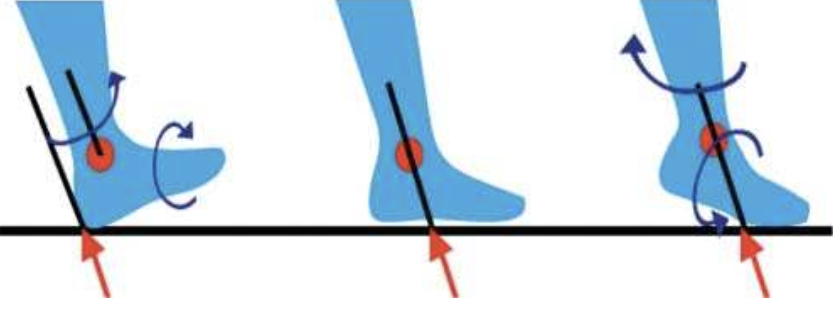
\includegraphics[width=0.65\textwidth]{images/movimiento_tibia_antepie.png}
    \caption{Movimiento en relación de tibia y antepié. Fuente: Sánchez Hernández et al. (2016), modificación de Viladot.}
    \label{fig:movimiento-tibia-antepie}
\end{figure}


Dentro de las lesiones por torsión del tren inferior, las lesiones de rodilla adquieren especial
relevancia por el papel de esta articulación en el soporte del peso corporal y en la
estabilización del movimiento. La rodilla debe responder a cargas provenientes tanto del cuerpo
como del contacto con el suelo, especialmente en situaciones de desaceleración, aterrizaje o
cambio de dirección. Cuando estas cargas se combinan con una alineación desfavorable, pueden
comprometer estructuras como ligamentos, meniscos y músculos que permiten la estabilización de
la rodilla \parencite{ShimokochiShultz2008,MakkiEtAl2022}.

Una de las lesiones más estudiadas dentro de este grupo es la lesión del ligamento cruzado
anterior. Este ligamento cumple un rol central en la estabilidad de la rodilla, particularmente
frente al desplazamiento anterior de la tibia y a ciertos movimientos de rotación. Las lesiones
sin contacto del ligamento cruzado anterior suelen asociarse con maniobras de aterrizaje o
desaceleración, donde la rodilla puede encontrarse cerca de la extensión y sometida a fuerzas
compresivas elevadas durante el apoyo \parencite{BodenSheehan2022}. A su vez, estas lesiones
también han sido vinculadas con acciones de desaceleración y cambio de dirección, en las que
pueden intervenir cargas combinadas sobre la rodilla \parencite{ShimokochiShultz2008}.

El análisis de estos mecanismos muestra que la lesión no suele depender de un único movimiento
aislado. En cambio, puede producirse por la combinación de fuerzas en distintos planos. A esto
se lo puede entender como una carga multiplanar: por ejemplo, una rodilla que recibe una fuerza
vertical de compresión, mientras al mismo tiempo se encuentra en rotación y con desplazamiento
hacia adentro o hacia afuera. En este sentido, \textcite{ShimokochiShultz2008} señalan que las
lesiones sin contacto del ligamento cruzado anterior tienden a involucrar cargas combinadas sobre
la rodilla, especialmente durante actividades con apoyo y desaceleración. De manera
complementaria, \textcite{BodenSheehan2022} destacan el papel de la carga axial compresiva como
componente principal en el mecanismo de lesión sin contacto del ligamento cruzado anterior,
mientras que la contracción del cuádriceps y las cargas laterales sobre la rodilla pueden
contribuir a aumentar la exigencia sobre el ligamento.

Además del ligamento cruzado anterior, los meniscos también pueden verse afectados en lesiones
de rodilla asociadas a la práctica deportiva. Estas estructuras contribuyen a la distribución de
cargas, la estabilidad articular y la absorción de impactos. En atletas, las lesiones meniscales
pueden afectar el rendimiento deportivo y presentarse en distintos contextos, incluyendo
mecanismos de contacto, no contacto o situaciones no específicas \parencite{MakkiEtAl2022}. Por
esta razón, al analizar lesiones por torsión del tren inferior, resulta pertinente considerar no
solo los ligamentos, sino también otras estructuras intraarticulares de la rodilla.

El tobillo constituye otra articulación relevante dentro de este tipo de lesiones, ya que
participa directamente en el contacto con el suelo y en la adaptación del cuerpo a distintas
superficies y direcciones de movimiento. Durante acciones deportivas, el tobillo debe permitir
movilidad y, al mismo tiempo, aportar estabilidad. Movimientos como la inversión del pie, es
decir, cuando la planta tiende a orientarse hacia adentro; la eversión, cuando la planta tiende
a orientarse hacia afuera; la flexión plantar, cuando el pie se dirige hacia abajo; y la
dorsiflexión, cuando el pie se aproxima a la tibia, pueden combinarse con rotaciones de la tibia
y cargas externas. Estas combinaciones generan situaciones de exigencia para las estructuras
ligamentarias y musculares del pie y del tobillo \parencite{SanchezHernandezEtAl2016}.

En este contexto, el concepto de lesión sin contacto resulta importante. Una lesión sin contacto
no implica necesariamente ausencia de carga, sino ausencia de un golpe directo como causa
principal. En muchos casos, la fuerza proviene del propio movimiento del deportista, de la
reacción del suelo, de la desaceleración del cuerpo o de una posición articular desfavorable
durante el apoyo \parencite{ShimokochiShultz2008}.

\subsection{Biomecánica del movimiento en el fútbol}

La biomecánica del movimiento en el fútbol permite estudiar cómo se organizan los segmentos
corporales y cómo actúan las fuerzas durante las acciones propias del juego. Su aplicación no
se limita al análisis del rendimiento, sino que también permite comprender la técnica deportiva,
las demandas físicas y los posibles factores asociados al riesgo de lesión. En el fútbol, esto
resulta especialmente relevante por la variedad de gestos que realiza el jugador durante un
partido o entrenamiento, como correr, acelerar, desacelerar, cambiar de dirección, saltar,
aterrizar, girar, disputar y golpear la pelota \parencite{PlakiasEtAl2024}.

El análisis biomecánico puede abordar variables cinemáticas y cinéticas. La cinemática permite
describir el movimiento a partir de posiciones, trayectorias, ángulos articulares, velocidades
lineales y velocidades angulares, sin analizar directamente las fuerzas que lo producen. En
cambio, la cinética se relaciona con las fuerzas que generan o modifican ese movimiento, como
las fuerzas de reacción del suelo o las fuerzas que generan un movimiento de rotación en las
articulaciones. En el fútbol, ambas dimensiones permiten estudiar acciones como los apoyos,
los cambios de ritmo, los desplazamientos, los saltos y los gestos técnicos
\parencite{CossioBolanosArruda2009}.

Los movimientos del fútbol suelen involucrar una interacción constante entre cadera, rodilla,
tobillo y pie. Durante un apoyo, la posición del pie puede modificar la orientación de la tibia
y, en consecuencia, influir sobre la alineación de la rodilla y la cadera. Esta relación es
importante porque muchas acciones del juego se realizan en apoyo monopodal, con cambios rápidos
de dirección o con el cuerpo rotando sobre una pierna. Por lo tanto, el análisis biomecánico del
fútbol requiere considerar al tren inferior como una cadena de segmentos interdependientes y no
como articulaciones aisladas \parencite{SanchezHernandezEtAl2016}.

Entre las acciones más relevantes para el análisis del tren inferior se encuentran las
desaceleraciones, los cambios de dirección, los saltos, los aterrizajes y los giros. Estas
acciones exigen que el jugador controle el centro de masa, estabilice la pierna de apoyo y
reorganice rápidamente la posición de sus segmentos corporales para continuar la acción. En
este tipo de gestos, la rodilla, el tobillo y la cadera deben coordinarse en tiempos breves,
mientras reciben cargas asociadas al peso corporal, la reacción del suelo y la rotación del
cuerpo \parencite{PlakiasEtAl2024}.

El golpeo de la pelota constituye otro gesto técnico relevante desde el punto de vista
biomecánico. Se trata de una acción de varias articulaciones en la que intervienen la pierna de
apoyo, la pierna de golpeo, la cadera, la rodilla, el tobillo, y todo lo que conforma el tronco.
\textcite{ManolopoulosEtAl2013} mencionan que el remate con empeine muestra que el rendimiento
del golpeo se relaciona con variables como la velocidad del pie, la velocidad angular de las
articulaciones, la activación muscular y las fuerzas de reacción del suelo.

El análisis biomecánico del fútbol también puede realizarse mediante métodos de medición
indirecta, como filmaciones o fotografías. Estos métodos permiten obtener información cinemática
a partir del registro visual del movimiento, como posiciones, trayectorias, velocidades y
aceleraciones de puntos o segmentos corporales. Si bien los métodos directos, como el estudio
por medio de laboratorio, pueden ofrecer mediciones más precisas de determinadas variables, el
video resulta especialmente útil por su cercanía con situaciones reales de entrenamiento y
competencia \parencite{CossioBolanosArruda2009}. En este sentido, los métodos indirectos y directos 
pueden considerarse complementarios: los primeros favorecen el análisis en contextos reales de juego, 
mientras que los segundos permiten obtener mediciones más controladas y precisas de determinadas variables

\subsection{Prevención de lesiones mediante el análisis del movimiento}

La prevención de lesiones en el fútbol no depende únicamente de conocer cuáles son las lesiones
más frecuentes, sino también de entender en qué situaciones y bajo qué patrones de movimiento
tienden a producirse. En este sentido, el análisis del movimiento permite observar cómo se
comporta el jugador durante acciones propias del juego. A partir de esta información, es posible
identificar condiciones biomecánicas o funcionales que podrían aumentar la exigencia sobre
determinadas estructuras del tren inferior \parencite{DellaVillaEtAl2020}.

En particular, el análisis de lesiones del ligamento cruzado anterior en fútbol profesional
muestra que muchas de estas lesiones no se producen por un golpe directo sobre la rodilla, sino
durante situaciones sin contacto directo o con contacto indirecto, siendo estas últimas
correspondientes a situaciones en las que existe contacto con el jugador, pero no directamente
sobre la rodilla lesionada. En estos casos, el jugador suele encontrarse realizando acciones como
presión defensiva, intento de quite, cambio de dirección, aterrizaje posterior a un salto o
recuperación del equilibrio luego de golpear la pelota \parencite{DellaVillaEtAl2020}. Algunas
de estas situaciones se representan de forma esquemática en la
Figura~\ref{fig:patrones_movimiento_futbol}.

\begin{figure}[H]
    \centering
    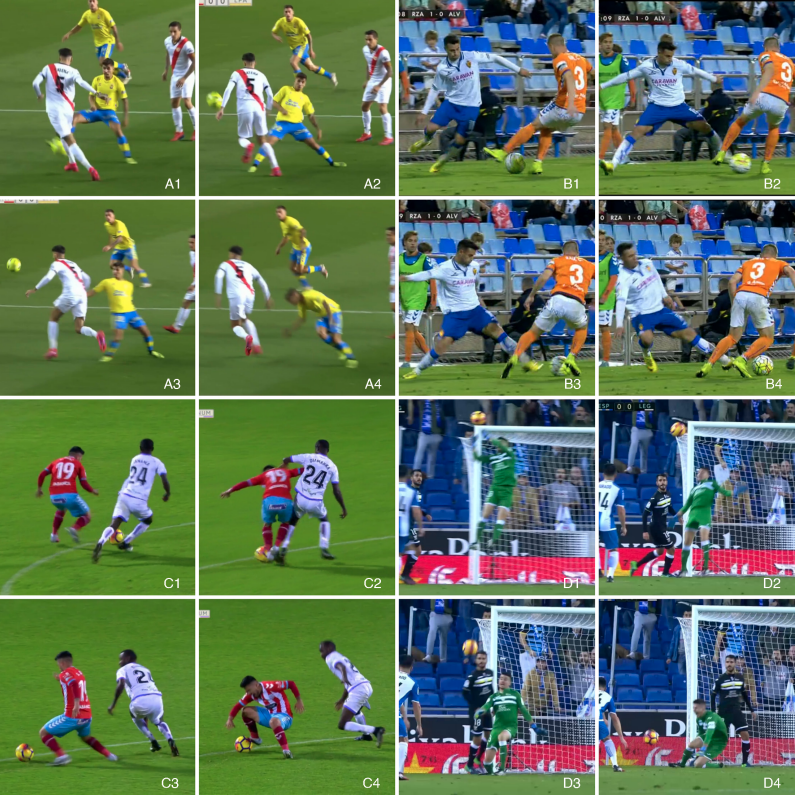
\includegraphics[width=0.85\textwidth]{images/patrones_movimiento_futbol.png}
    \caption{Patrones situacionales principales asociados a lesiones del ligamento cruzado
    anterior en fútbol profesional.
    (A) Presión (\textit{pressing}) (jugador con camiseta amarilla, lesión del LCA derecho):
    aproximación/presión sobre el oponente (A1), contacto inicial del pie derecho con el suelo
    (A2), instante estimado de lesión del LCA derecho (A3), pérdida del equilibrio (A4).
    (B) Quite o entrada defensiva (\textit{tackling}) (jugador con camiseta blanca, lesión del
    LCA derecho): aproximación/presión sobre el oponente (B1), contacto inicial del pie derecho
    con el suelo e intento de quite (B2), instante estimado de lesión del LCA derecho (B3),
    pérdida del equilibrio (B4).
    (C) Ser tackleado o recibir la entrada del rival (\textit{being tackled}) (jugador con
    camiseta roja, lesión del LCA derecho): presión ejercida por el jugador oponente (C1),
    perturbación mecánica/contacto del jugador defensor (C2), instante estimado de lesión del
    LCA derecho (C3), pérdida del equilibrio (C4).
    (D) Aterrizaje tras un salto (\textit{landing from a jump}) (arquero, uniforme verde, lesión
    del LCA derecho): salto (D1), contacto inicial de ambos pies con el suelo (D2), instante
    estimado de lesión del LCA derecho (D3), pérdida del equilibrio (D4).
    LCA: ligamento cruzado anterior. Fuente: adaptado de \textcite{BuckthorpeEtAl2024ACL}.}
    \label{fig:patrones_movimiento_futbol}
\end{figure}


El análisis preventivo del movimiento busca observar variables que puedan aportar información
sobre la calidad del gesto deportivo. Entre ellas se encuentran la alineación de la rodilla, la
posición del pie durante el apoyo, la orientación de la cadera, el control del tronco, la
estabilidad en apoyo monopodal\footnote{Apoyo monopodal: situación en la que el cuerpo se
sostiene principalmente sobre una sola pierna.}, la simetría entre miembros y la forma en que
el jugador absorbe o redirige las cargas. Estas variables no permiten afirmar que una lesión vaya
a ocurrir, pero sí pueden ayudar a detectar patrones que conviene revisar dentro de un programa
de entrenamiento, prevención o readaptación
\parencite{DellaVillaEtAl2020,BuckthorpeEtAl2024ACL}.

Los estudios basados en videoanálisis resultan especialmente útiles porque permiten estudiar
lesiones reales dentro del contexto del juego. A diferencia de una evaluación de laboratorio o
de un test funcional controlado, el video de partido o entrenamiento permite observar la
interacción entre el jugador, el oponente, la pelota, la velocidad de la acción y las decisiones
tomadas en tiempos muy breves. En este sentido, \textcite{BuckthorpeEtAl2024ACL} y
\textcite{BuckthorpeEtAl2025Ankle} utilizaron este tipo de análisis para describir mecanismos
de lesión, patrones situacionales, características biomecánicas y factores neurocognitivos
asociados a lesiones del ligamento cruzado anterior y del tobillo en futbolistas profesionales.

Desde una perspectiva preventiva, el valor del análisis de movimiento se encuentra en su
capacidad para generar información observable y accionable. Por ejemplo, si durante una
desaceleración o un cambio de dirección se observa una rodilla que tiende al
valgo\footnote{Valgo: desviación de un segmento corporal hacia la línea media del cuerpo. En la
rodilla, el valgo suele observarse cuando esta se desplaza hacia adentro respecto de la cadera y
el pie.}, un apoyo inestable del pie, una caída con poco control de cadera o una pérdida de
estabilidad del tronco, esa información puede ser utilizada por profesionales del cuerpo técnico
o médico para orientar ejercicios de fuerza, estabilidad, coordinación, técnica de aterrizaje o
control neuromuscular\footnote{Control neuromuscular: capacidad del sistema nervioso y muscular
para coordinar la activación de los músculos y estabilizar las articulaciones durante el
movimiento.}. En la Figura~\ref{fig:valgo_dinamico} se muestran algunas de las variables
observables del tren inferior que pueden considerarse en este tipo de análisis
\parencite{DellaVillaEtAl2020,BuckthorpeEtAl2024ACL}.

\begin{figure}[H]
    \centering
    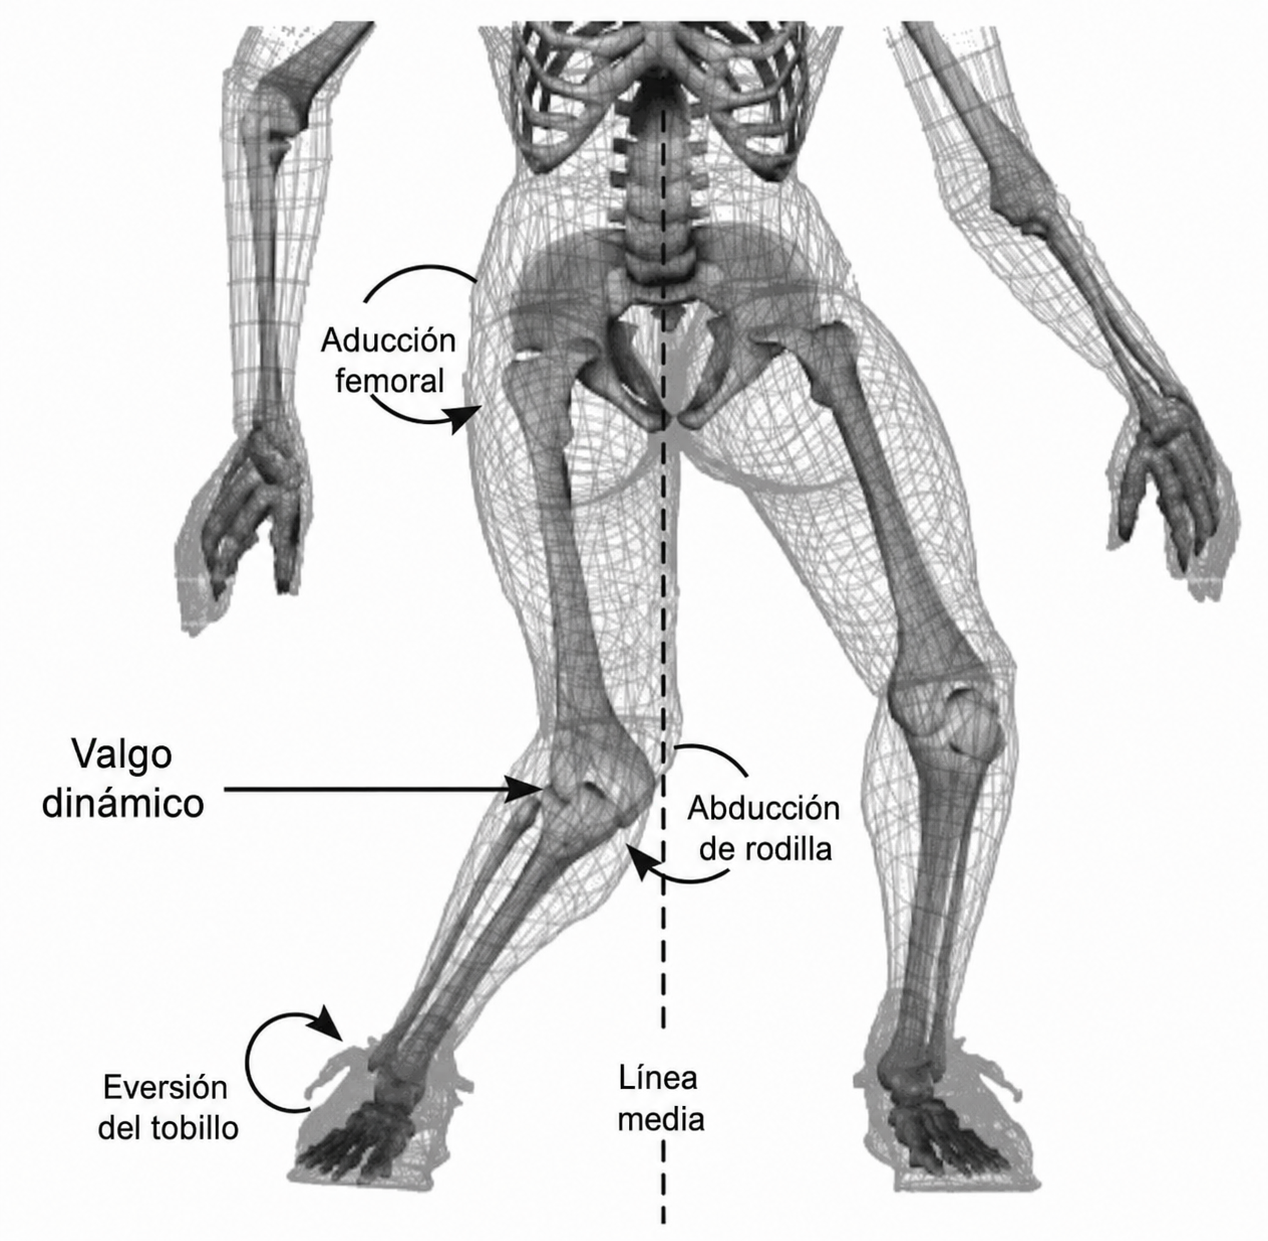
\includegraphics[width=0.55\textwidth]{images/valgo_dinamico.png}
    \caption{Representación esquemática del valgo dinámico y la alineación del miembro inferior.
    Fuente: adaptado de \textcite{HewettEtAl2005} (p.~494), con rediseño y traducción al español
    asistidos por IA.}
    \label{fig:valgo_dinamico}
\end{figure}


Sin embargo, es importante considerar que la relación entre movimiento y lesión no es lineal ni
determinística. Una evaluación funcional o biomecánica puede aportar información relevante, pero
no permite predecir con certeza qué jugador se lesionará. De hecho, algunos estudios sobre
herramientas de evaluación funcional en futbolistas señalan que ciertos métodos deben utilizarse
con cautela cuando se los interpreta como predictores directos de lesiones sin contacto
\parencite{SmithHanlon2017}. Por esta razón, el análisis del movimiento debe entenderse como un
recurso complementario dentro de un enfoque más amplio, que también considere la carga de
entrenamiento, el historial de lesiones, la fatiga, la fuerza, la movilidad, el contexto de
juego y la intervención profesional.

\subsection{Inteligencia artificial aplicada al deporte}

Completar.

\subsection{Visión por computadora}

Completar.

\subsection{Estimación de postura humana}

Completar.

\subsection{Machine learning aplicado al análisis de movimiento}

Completar.

\input{chapters/conclusion}

\addcontentsline{toc}{chapter}{Bibliograf\'{\i}a}
\printbibliography{}

\appendix
\input{chapters/appendix/annex}

\newpage
\listoffigures

\newpage
\listoftables

\end{document}